\documentclass{article}
\usepackage[utf8]{inputenc}
\usepackage{geometry}
\usepackage{hyperref}
\usepackage{multicol}
\usepackage{graphicx}

 \geometry{
 a4paper,
 total={170mm,257mm},
 left=20mm,
 top=20mm,
 }
 \usepackage{graphicx}
 \usepackage{titling}

 \title{Group A3D: RDF Dataset}
\author{Group A3D}
\date{20th December 2024}

 \usepackage{fancyhdr}
\fancypagestyle{plain}{%  the preset of fancyhdr
    \fancyhf{} % clear all header and footer fields
    % \fancyfoot[R]{\includegraphics[width=2cm]{KULEUVEN_GENT_RGB_LOGO.png}}
    \fancyhead[]{\thedate}
    \fancyhead[L]{RDF Dataset}
    \fancyhead[R]{\theauthor}
}
\makeatletter
\def\@maketitle{%
  \newpage
  \null
  \vskip 1em%
  \begin{center}%
  \let \footnote \thanks
    {\LARGE \@title \par}%
    \vskip 1em%
    %{\large \@date}%
  \end{center}%
  \par
  \vskip 1em}
\makeatother

\usepackage{lipsum}
\usepackage{cmbright}

\begin{document}

\maketitle

\noindent\begin{tabular}{@{}ll}
	\textbf{Group members:}
  & \href{mailto:andrea.bruttomesso.1@studenti.unipd.it}{Andrea Bruttomesso} 2120933\\
	& \href{mailto:alessandro.corro.1@studenti.unipd.it}{Alessandro Corr\`o} 2125034\\
	& \href{mailto:davide.seghetto@studenti.unipd.it}{Davide Seghetto} 2122548\\
	& \href{mailto:andrea.stocco.8@studenti.unipd.it}{Andrea Stocco} 2108885\\
\end{tabular}
\\\\\\
\noindent\begin{tabular}{@{}ll}
	\textbf{Link to the GitHub repository:} \href{https://github.com/andreastocco01/a3d}{https://github.com/andreastocco01/a3d}
\end{tabular}

\section*{Mapping of the open data in RDF}
We modeled an ontology that captures the relationships among three key domains: Nobel Prize winners, academic papers published in journals or conferences,
and R\&D (research and development) budgets allocated by nations over the years. By integrating these domains, the ontology provides a comprehensive
framework to explore connections between outstanding scientific discoveries, scholarly output, and the financial investments that drive global innovation.
This integrated approach enables a deeper understanding of the dynamics between scientific achievement and the resources that fuel it, highlighting how
funding decisions may influence groundbreaking research and its impact on society. Through this process, we aim to create a valuable resource for
researchers and scholars, offering a clearer view of the intersection between scientific achievements, academic output, and the financial investments
that drive progress in various fields of knowledge.

\noindent In order to model our ontology, we utilized four distinct open
datasets, which contain information regarding Nobel Prize winners, scientific papers, scientific journals, and investments in R\&D by countries.

\noindent We mapped the data into RDF format in the following way.

\begin{figure}[ht]
    \centering
    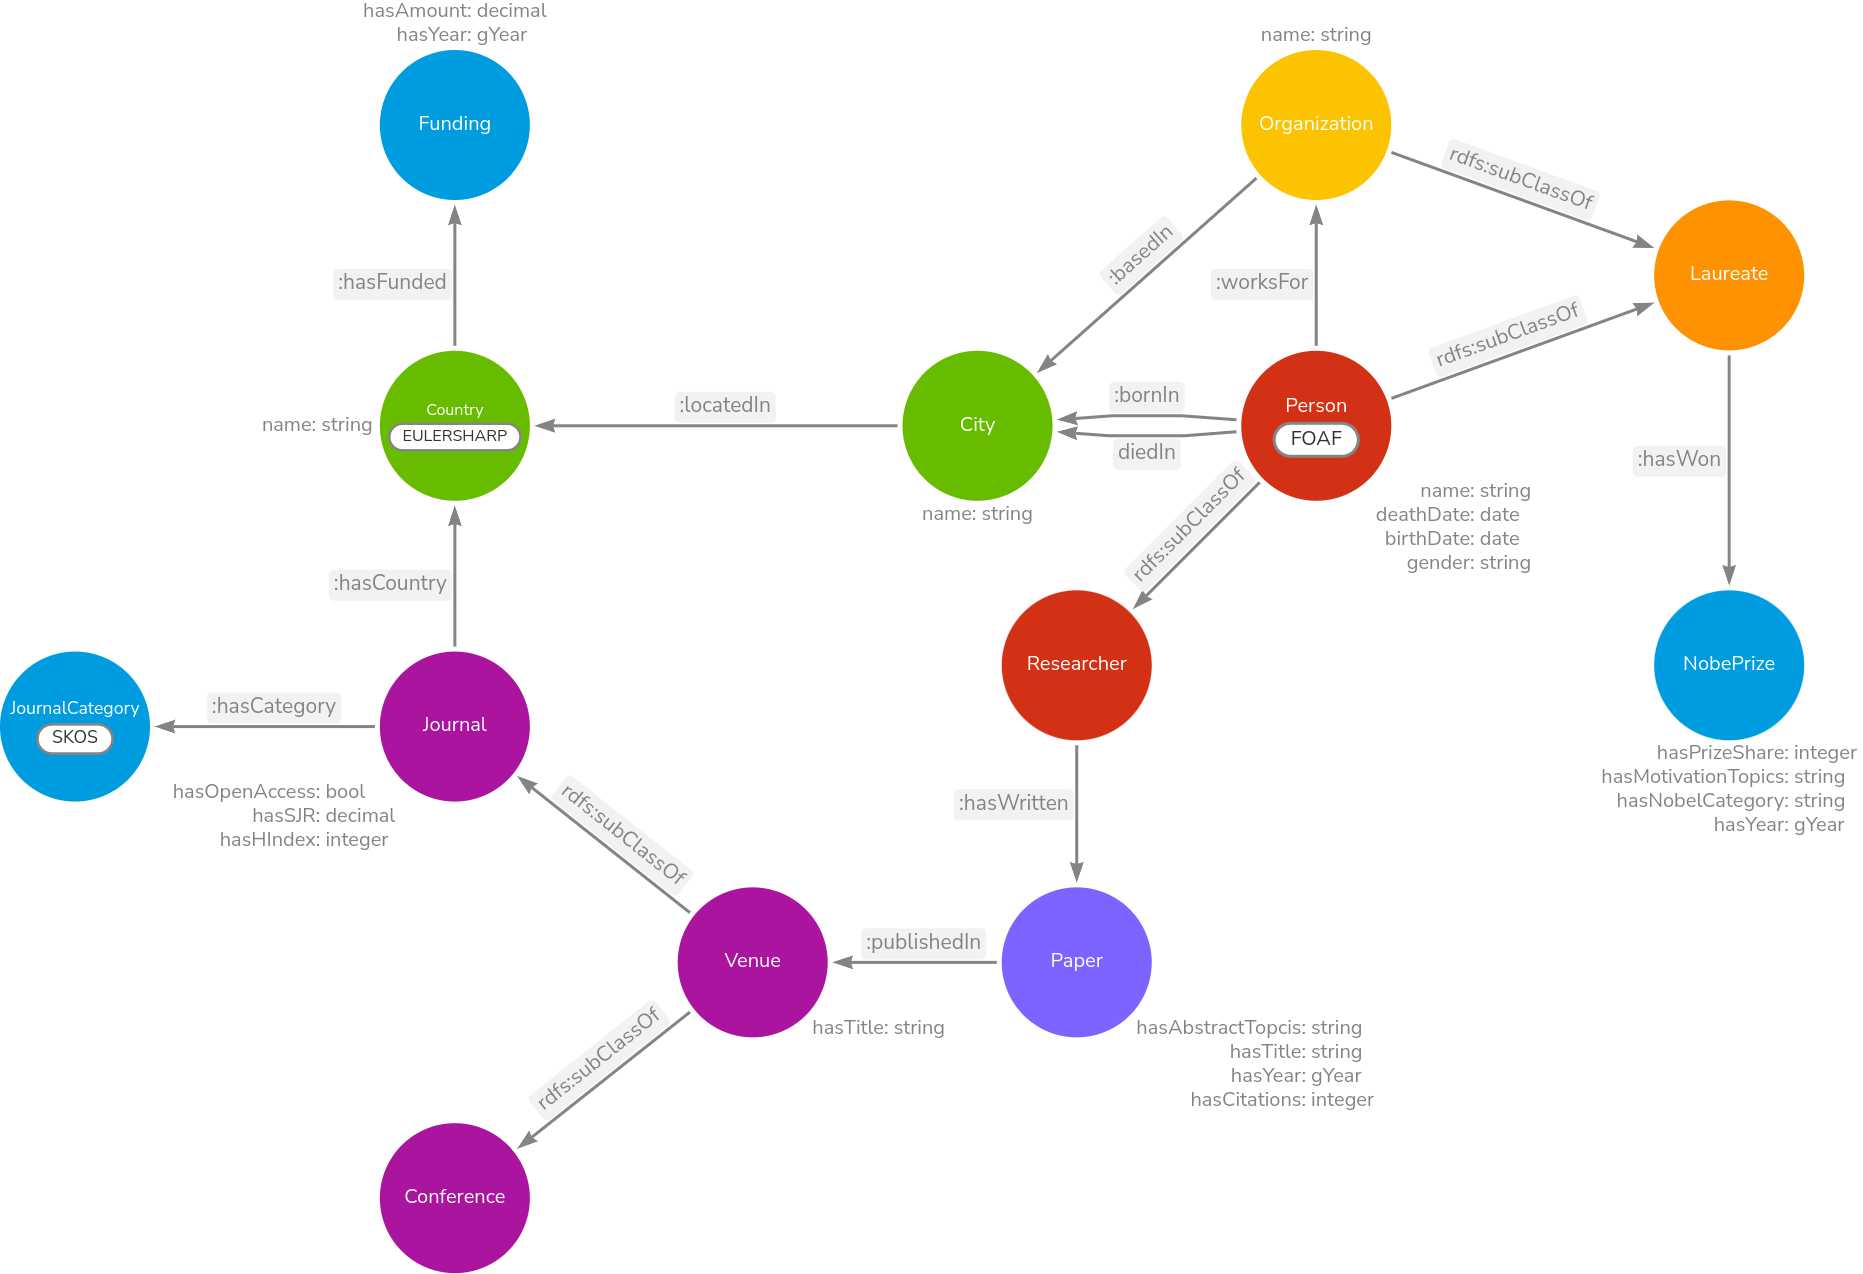
\includegraphics[width=\textwidth]{nobelOntologyTransparent.png}
    \caption{nobelOntology}
    \label{fig:nobelOntology}
\end{figure}

\newpage

\noindent We had to address the issue of duplicates to ensure that there were no resources in the RDF dataset with the same URI representing the same
entity. This is a critical aspect of maintaining data integrity and avoiding inconsistencies in the ontology. Therefore, before adding a new resource to
the RDF dataset, such as a scientific journal, we performed a thorough check to confirm that the resource was not already present in the graph.
To facilitate this, we defined a series of functions, such as \textit{handle\_city} and \textit{handle\_org}.

\noindent In addition to addressing duplicates, we also encountered the challenge of discrepancies in naming conventions between the data in our open
datasets and the EulerSharp ontology. In particular, some country names in our datasets differed from those used in the EulerSharp ontology, e.g. "United
States" and "United States of America", so we had to manually handle these specific cases.

\noindent In addition, we wrote a script (\textit{topic\_extraction.py}) to extract the most significant words from the texts that define the abstract of a
scientific paper and the motivation for the award of a Nobel Prize. The script was developed to generate shorter, more concise values for properties
\textit{motivationAbstract} and \textit{motivationTopics}. For instance, long descriptions such as "in recognition of the extraordinary services he has rendered by the
discovery of the laws of chemical dynamics and osmotic pressure in solutions" are transformed into more focused terms like "chemical dynamics osmotic
pressure solutions." This approach enhances the dataset's efficiency by reducing the length of textual values while preserving the key concepts relevant
to the Nobel Prize motivation and the research topics.

%\subsection*{Nobel Prize Dataset}
%We processed the Nobel Prize data to create RDF triples that represent laureates, the Nobel Prize they won, and the related metadata
%(e.g., year, category, motivation etc.). In particular, for the URI creation of the Nobel laureates we used the ontology base URI and their name 
%(e.g. the URI for Albert Einstein is \url{http://www.semanticweb.org/a3d/ontologies/2024/10/nobelOntology/AlbertEinstein}), while for the URI of the Nobels
%we used the ontology base URI and the category of the prize followed by the year of award (e.g. the URI for the Nobel Prize in Chemistry of 1956
%is \url{http://www.semanticweb.org/a3d/ontologies/2024/10/nobelOntology/Chemistry1956}).
\section*{Main Statistics}

The following statistics summarize the key features of the RDF dataset created from the ontology.

\begin{itemize}
    \item \textbf{Entity and Triple Counts:}
    \begin{itemize}
        \item Total number of RDF triples: 207,258
        \item Number of unique entities:
        \begin{itemize}
            \item Person: 6,677
            \item Researchers: 4,919
            \item Laureates: 1,785
            \item Organizations: 355
            \item Papers: 5,002
            \item Journals: 18,616
            \item Conferences: 306
            \item Cities: 881
            \item Countries: 246
            \item Nobel Prizes: 581
            \item Funding: 2,747
        \end{itemize}
    \end{itemize}
    
    \item \textbf{Laureates and Nobel Prizes:}

    The dataset contains information about Nobel Prizes awarded from 1901 to 2016.
    \begin{itemize}
        \item Total Nobel Prizes awarded: 581
        \item Prize categories: Physics, Chemistry, Medicine, Literature, Peace, Economics
        \item Gender distribution of laureates:
        \begin{itemize}
            \item Male: 1664 (94.6\%)
            \item Female: 94 (5.4\%)
        \end{itemize}
        \item Researchers that won a Nobel Prize: 1
        \item Organizations that won a Nobel Prize: 29
        \item Most awarded countries: 

        \vspace{0.5cm}
        \hspace{2cm}
        \begin{tabular}{|c|l|c|}
          \hline
          \textbf{Position} & \textbf{Country} & \textbf{Total prizes} \\
          \hline
          1 & United States of America & 514 \\
          \hline
          2 & United Kingdom & 198 \\
          \hline
          3 & Germany & 160 \\
          \hline
          4 & France & 146 \\
          \hline
          5 & Italy & 129 \\
          \hline
        \end{tabular}
    \end{itemize}
    
\end{itemize}

\end{document}
